\section{GARCH}
\subsection{Model Justification}
Volatility in financial markets is a key indicator for assessing risk and is crucial in forecasting future values. The sanctions imposed on Russia following its invasion of Ukraine on 24 February 2022 heavily impacted the European energy market as Russia was the main supplier of natural gas in the region. Extreme volatility in the energy market has been observed since, as the market responds to these ongoing sanctions. When looking closely at the Australian energy market to assess the responses of the domestic natural gas and crude oil markets to Russian sanctions, historic volatility modelling is useful in helping us predict how the markets would have performed sans sanctions.
\medskip

The LNG and oil markets are inherently volatile commodities as they are primarily driven by market-specific demand and supply shocks as well as structural shocks. The nature of the markets means that we cannot assume a state of constant volatility as the prices fluctuate based on specific forces. Extensive literature review has shown that on forecasting commodities such as natural gas and crude oil, recent studies have commonly used models that allow for regime switching after a certain threshold such as Self-Exciting Threshold AutoRegressive (SETAR) and variations of Generalised Autoregressive Conditional Heteroskedasticity (GARCH) models \cite{alice1}. For example, Ngyuen and Nabney \cite{alice2} used GARCH models combined with linear regressions and Artificial Neural Networks (ANN) to forecast natural gas prices; Lv and Shan \cite{alice3} used non-linear GARCH type models as part of their analysis and research into the volatility of natural gas prices. There is a clear precedence of the usage of econometric models, in particular GARCH model variations, in analysing the volatility of commodities such as natural gas and crude oil in practice, which sets the stage for the model selected in this project.
\medskip

The GARCH model is designed to help produce a measure for volatility. These autoregressive processes depend on past observations and variances in modelling for current and future variances. A feature of the GARCH model that makes it relevant to use in forecasting energy markets such as LNG and crude oil is that these models do not assume constant volatility. For a more realistic model, GARCH models are designed in a Bayesian framework with a learning behaviour in place to use the most recent standard deviation of returns. By aiming to minimise prediction errors by accounting for errors in prior forecasting, the accuracy of the predictions is more enhanced, which is why a GARCH model was selected for forecasting LNG and crude oil prices.

\subsection{GARCH Model: GSH Market}

The dataset contains 8 columns of data, however only 2 are needed: the trade data and the price of the trade. Once we have filtered these columns, we need to create a new column for the percent change for the day-to-day prices. These measures were done using the Pandas library in Python. 
\medskip

The returns on the prices were then squared under an additional column for running the GARCH model fit on.
\begin{figure}[H]
    \centering
    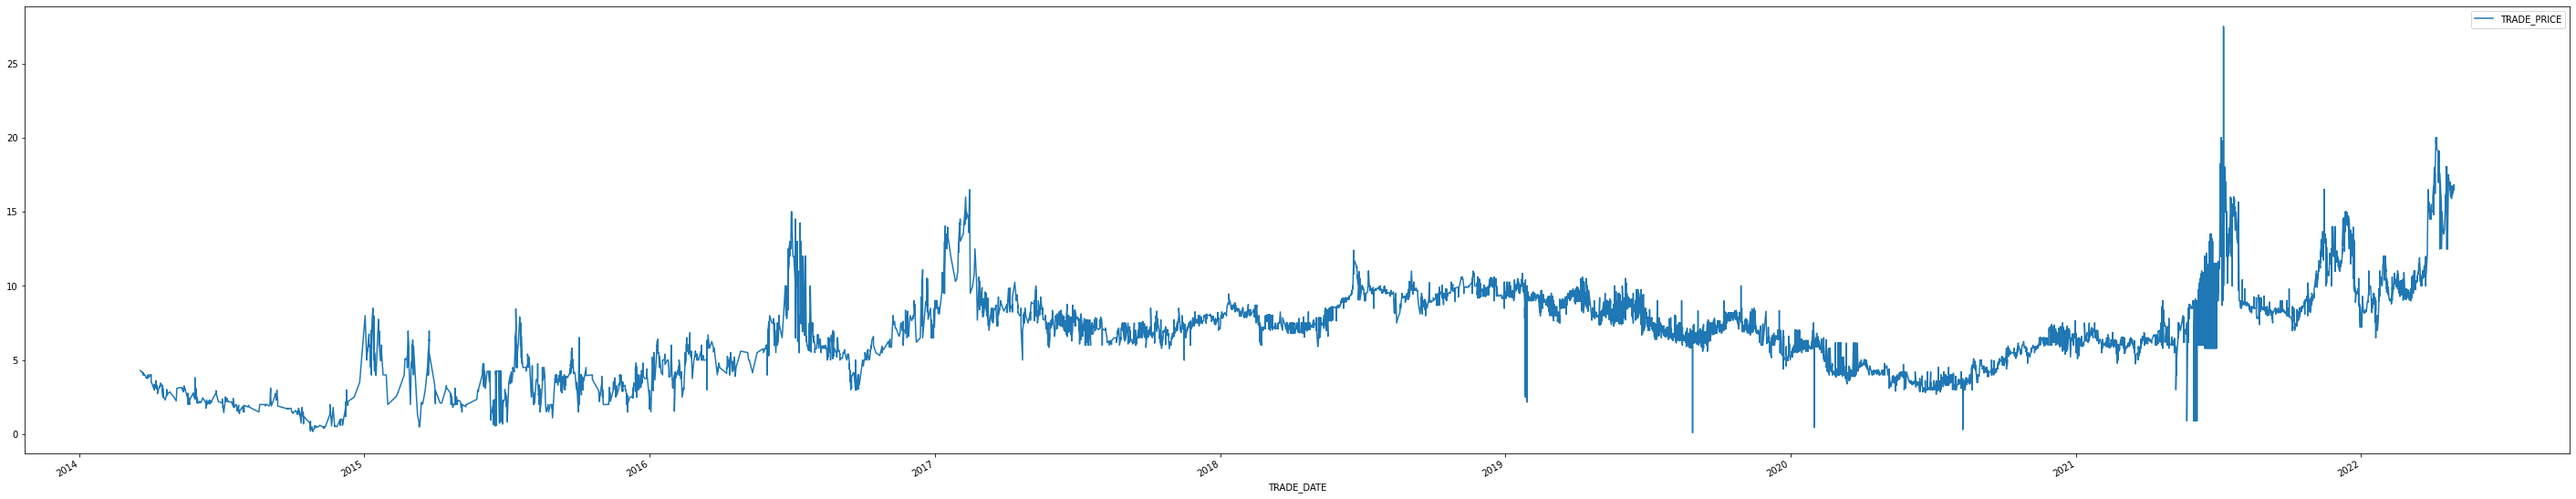
\includegraphics[width=1.0\textwidth]{Figures/Garch/gas.png}
    \caption{Daily GSH Returns Plot}
    \label{fig:Results_table}
\end{figure}

We found a GARCH(1, 1) model to fit the best, obtaining statistically significant p-values and t-test scores, as well as a relatively low AIC and BIC when compared to other GARCH mode parameters.
\begin{figure}[H]
    \centering
    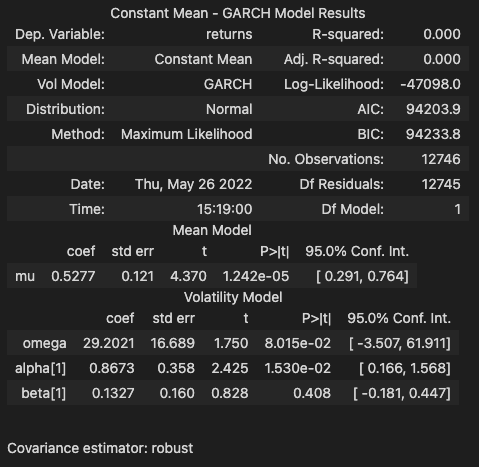
\includegraphics[width=0.5\textwidth]{Figures/Garch/garch.png}
    \caption{GARCH(1, 1) for GSH Market}
    \label{fig:Results_table}
\end{figure}

\subsection{GARCH Model: Brent Crude Oil}
\begin{figure}[H]
    \centering
    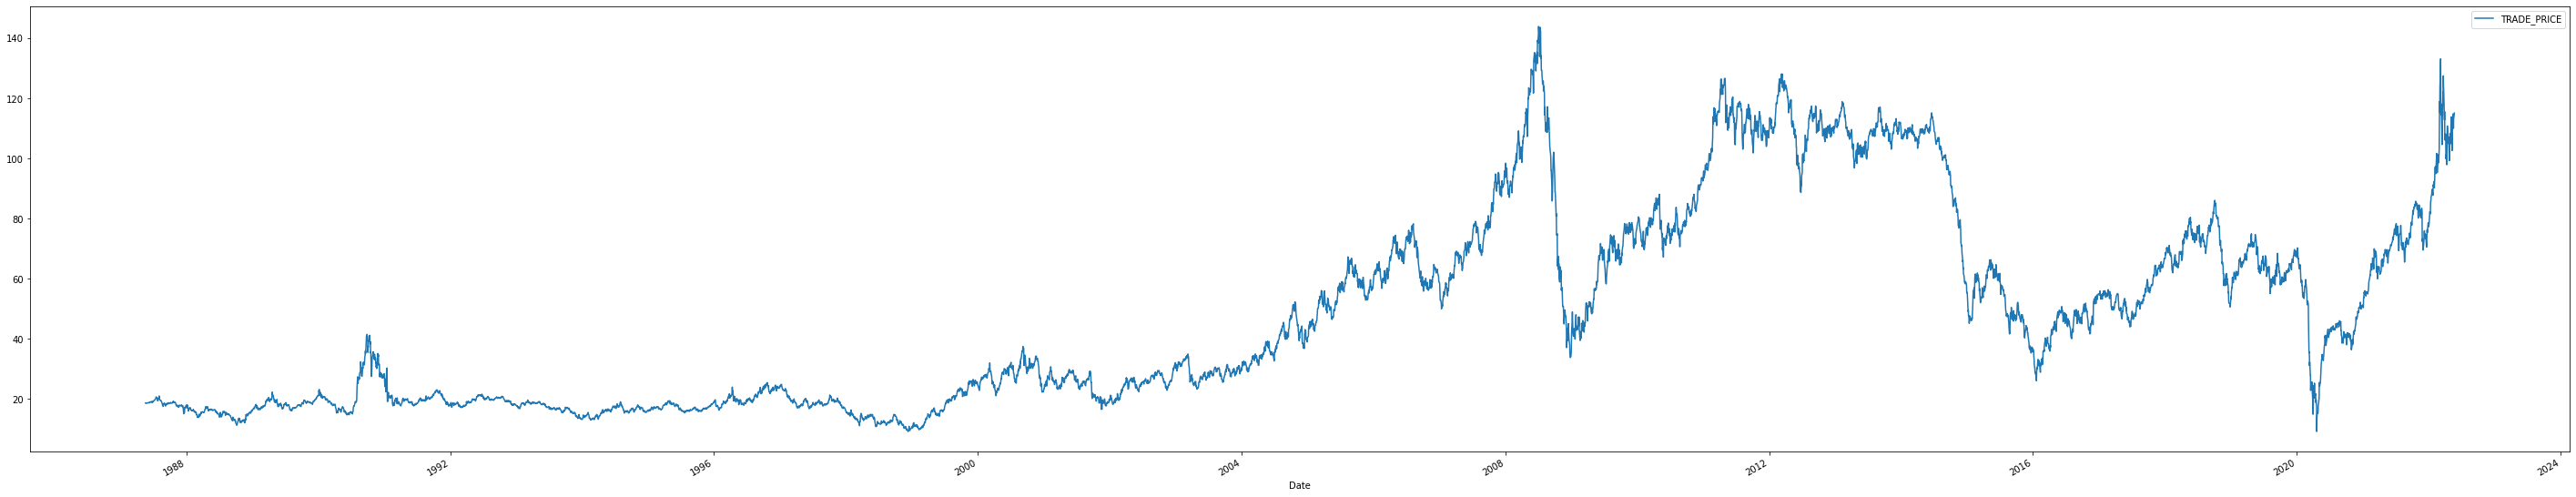
\includegraphics[width=1.0\textwidth]{Figures/Garch/brent.png}
    \caption{Daily Brent Crude Oil Returns (Dollar per Barrel) Plot}
    \label{fig:Results_table}
\end{figure}
The data for crude oil was of a daily frequency and did not need much wrangling or modification for the model. However, we created a column for daily percent returns for the price on dollars per barrel of crude oil. Following the same process as the GSH data, we were able to attain a GARCH(1, 1) model with competent p-value and t-test values as well as a low AIC and BIC. 
\medskip

\begin{figure}[H]
    \centering
    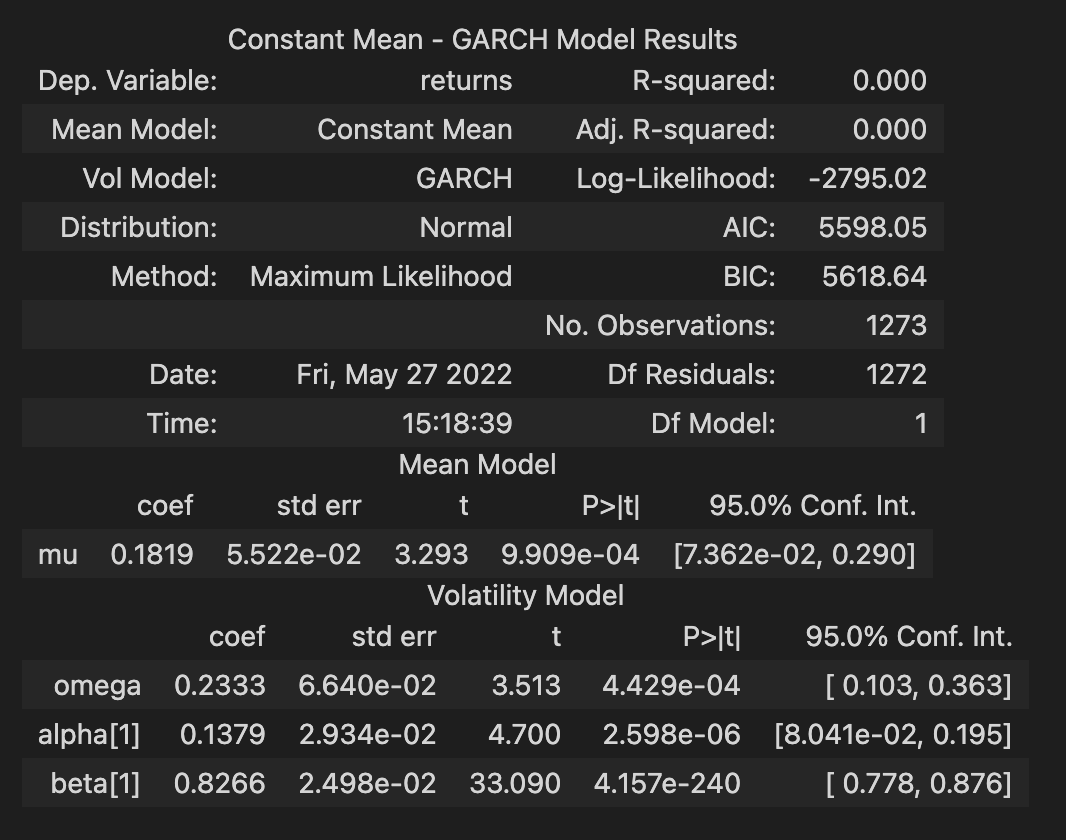
\includegraphics[width=0.5\textwidth]{Figures/Garch/crude.png}
    \caption{GARCH(1, 1) Model for Brent Crude Oil Market}
    \label{fig:Results_table}
\end{figure}

\subsection{Annualised Conditional Volatility}
The following are the standardised residuals and the annualised conditional volatility for the GSH Market and the Brent Crude Oil Market:
\begin{figure}[H]
\centering
\begin{minipage}{.5\textwidth}
  \centering
  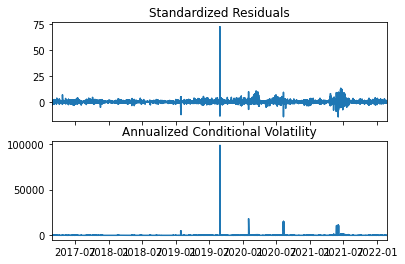
\includegraphics[width=1.0\linewidth]{Figures/Garch/gas_annualised.png}
  \label{fig:test1}
\end{minipage}%
\begin{minipage}{.5\textwidth}
  \centering
  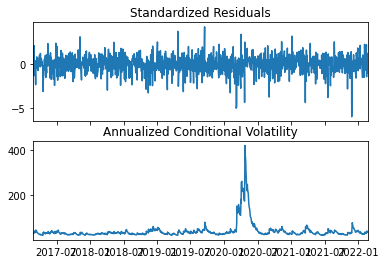
\includegraphics[width=1.0\linewidth]{Figures/Garch/crude_annualised.png}
  \label{fig:test2}
\end{minipage}
\end{figure}

\subsection{Forecasting Volatility}
We then mapped the volatility and forecasted it for the remainder of each of the datasets past the date of the Russian sanctions being imposed. For the Gas Supply Hub this was 68 days of forecasting and 91 days for the Brent Crude Oil. We mapped this forecast along with the volatility of the realised values of both datasets.
\begin{figure}[H]
    \centering
    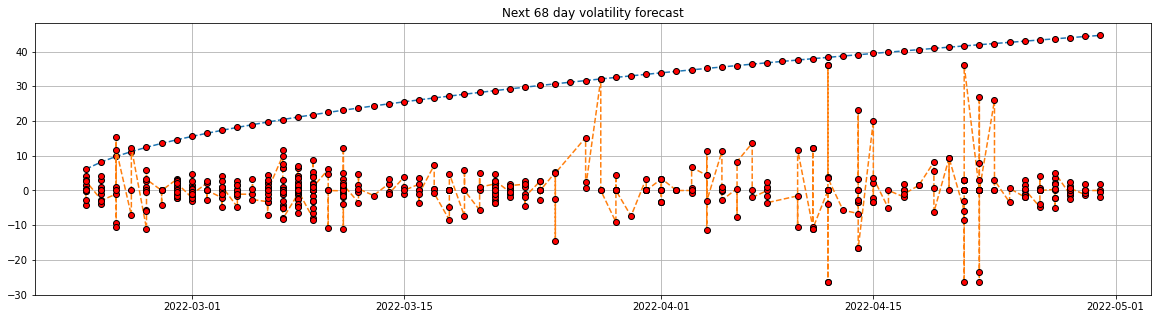
\includegraphics[width=0.6\textwidth]{Figures/Garch/gas_forecast.png}
    \caption{GSH Market Volatility Forecast with Realised Values}
    \label{fig:Results_table}
\end{figure}
\begin{figure}[H]
    \centering
    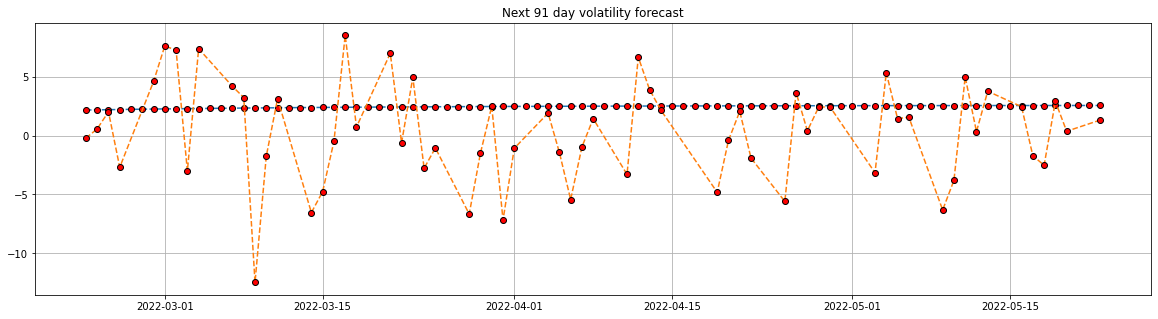
\includegraphics[width=0.6\textwidth]{Figures/Garch/crude_forecast.png}
    \caption{Brent Crude Oil Market Volatility Forecast with Realised Values}
    \label{fig:Results_table}
\end{figure}

As we can see,  there is a better fit for the trend of volatility for the GSH as opposed to the Brent Crude Oil, which is far more volatile in nature. This aligns with our initial hypothesis as the Gas Supply Hub market is more domestic in nature of trades and since most of the gas in Australia is mined and stored within Australian soil, the export is well regulated after meeting national demand. However, Brent Crude Oil is a more international market consisting of multiple European nations that rely heavily on the imports of natural gas for their industries, with a large supplier for these demands being Russia. Hence, it is expected for our GARCH forecast to underestimate the volatility of the market post-sanctions. 